\documentclass{beamer}
\usepackage{otf}
\usepackage{graphicx}
% Beamer 設定
\usetheme{default}
\usefonttheme[onlymath]{serif}
\setbeamertemplate{navigation symbols}{}
\renewcommand{\kanjifamilydefault}{\gtdefault}
\mathversion{bold}
% タイトル定義
\title{統計処理及び機械学習に基づく\\データマイニング入門\\第2回}
\author{宮本 隆志}
\institute{ナビプラス株式会社}
\date{\today}
% 文書開始
\begin{document}
% タイトルページ
\begin{frame}
  \titlepage
\end{frame}
% この勉強会について
\begin{frame}
  \frametitle{この勉強会について}
  \begin{itemize}
    \item データマイニングの入門講座です。
    \begin{itemize}
      \item 想定する聴衆は、これからデータを解析してみようという初学者を想定しています。
      \item 専門家や既に実務経験の豊富な方々には物足りない内容かと思います。
    \end{itemize}
    \item データマイニング = 
    \begin{itemize}
      \item 大量のデータを
      \item 統計学や機械学習などの手法を用いて探索・分析して
      \item 意味あるパターンやルールを発見する
    \end{itemize}
    と考えます。この勉強会では手法の話をします。
    \item ツールは無料のオープンソースのものを使用します
    \begin{itemize}
      \item メインにPythonを使用します。Anaconda-2.1.0 を用いて説明します。
    \end{itemize}
    \item 参考書はイベントWebページには記載しましたが、あまり準拠しません。
    \begin{itemize}
      \item あまり準拠すると著作権的に問題があるので。
    \end{itemize}
  \end{itemize}
\end{frame}
% 自己紹介
\begin{frame}[containsverbatim]
  \frametitle{自己紹介}
  \begin{description}
    \item[名前] 宮本 隆志 ( @tmiya\_ )
    \item[所属/仕事] ナビプラス株式会社 / データ解析周りのR\&Dの仕事
    \item[ナビプラス] マーケティングソリューションツールの開発・提供
    \begin{itemize}
      \item サイト内検索エンジン・レコメンドエンジン、レヴュー投稿エンジンが中心
      \item 次世代インターネットサービスの研究・開発
      \item 上記に付随する広告商品の販売
    \end{itemize}
    \item[前職] ネット広告の入札サーバを開発する会社で似たような仕事
    \item[興味] 機械学習 / 関数型言語 / 定理証明系
    \begin{itemize}
      \item Coqという定理証明系の勉強会を毎月開催しています
    \end{itemize}
  \end{description}
\end{frame}
% 勉強会の進め方
\begin{frame}
  \frametitle{勉強会の進め方:予定}
  \begin{itemize}
    \item 講義(30分 + 30分) + 実習(40分) の形式。
    \item 前半は統計処理とか機械学習の手法の講義を中心。
    \begin{itemize}
      \item 前回分へのご意見を元に、演習資料の説明時間を増やすことにしました。
    \end{itemize}
    \item 後半はPythonを用いて簡単なハンズオンを予定。
    \begin{itemize}
      \item 興味のない方は講義について質問したり退出したりPython以外で解析するとかでお願いします。
      \item Python環境はAnaconda-2.1.0を推奨しますが、各自に任せます。
      \item ハンズオン用ファイル配布のために、Pythonの他にgitも導入してください。(あるいはUSBメモリでファイルを配布します。)
    \end{itemize}
    \item 講義形式の勉強会とは別に、読書会(教科書とか論文とか)とかやりたいので興味のある方、別途相談しましょう。
  \end{itemize}
\end{frame}
% 参考文献
\begin{frame}
  \frametitle{今回の内容}
  今回話す内容
  \begin{itemize}
    \item 検定の基礎
    \item $\chi^2$ 検定
  \end{itemize}
  今回話さない内容 $\Rightarrow$ 次回に回します
  \begin{itemize}
    \item $\chi^2$ 検定の別な例:Bradley-Terry モデル
    \item 多腕バンディット問題
  \end{itemize}
\end{frame}
% 参考文献
\begin{frame}
  \frametitle{参考文献}
  検定の話は、きちんとした話をするのは大変なので、教科書を読んで勉強したほうが良いと思います。\\
  \begin{itemize}
    \item 統計学:各自お好きな教科書で。
    \begin{itemize} 
      \item 東京大学教養学部統計学教室編 基礎統計学 I ~ III 「統計学入門」「自然科学の統計学」「人文・社会科学の統計学」
    \end{itemize}  
    \item 検定(特にサンプルサイズの話)
    \begin{itemize}
      \item 豊田秀樹「検定力分析入門」:R を使った入門書です。
      \item 永田靖「サンプルサイズの決め方」
      \item 大久保・岡田「伝えるための心理統計」
    \end{itemize}
  \end{itemize}
\end{frame}
% ファイル取得
\begin{frame}[fragile]
  \frametitle{ハンズオンファイルの取得}
  ハンズオンファイルの取得方法
  \begin{itemize}
    \item 初めての人は適当な作業用ディレクトリで(下記を1行で) \\ \texttt{\$ git clone https://github.com/} \texttt{takashi-miyamoto-naviplus/spml4dm.git} \\を行ってください。
    \item 既に \texttt{git clone} している人は、\texttt{spml4dm/} ディレクトリで、\\ \texttt{\$ git pull} \\ して下さい。
    \item git を導入してない場合は、USB メモリにてファイルを配布します。
  \end{itemize}
  IPython 起動方法
  \begin{itemize}
    \item \texttt{spml4dm/2/} ディレクトリに移動して、\\
    \texttt{\$ ipython notebook}
  \end{itemize}
\end{frame}
% IPython
\begin{frame}
  \frametitle{IPython}
  \texttt{spml4dm/2/} ディレクトリに移動 $\Rightarrow$ \\
  \texttt{\$ ipython notebook} \\
  $\Rightarrow$ Home画面:ノートブック選択 or 新規作成 $\Rightarrow$ 
  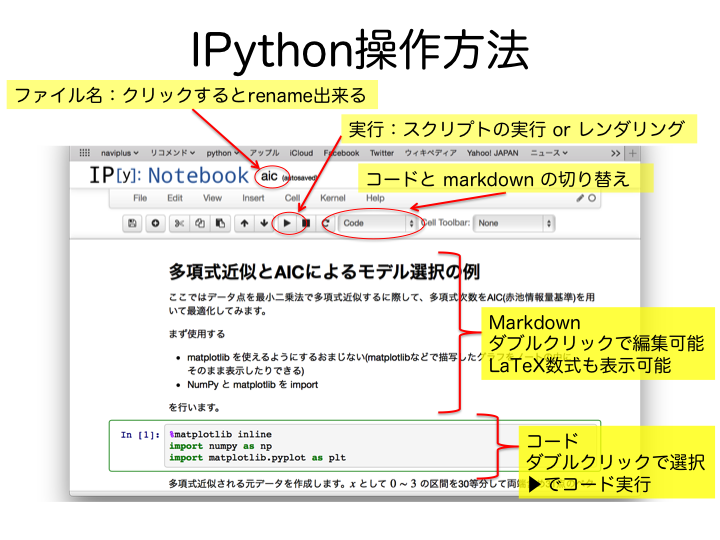
\includegraphics[clip, width=\textwidth, natwidth=720, natheight=540, trim=0 0 0 75]{ipython_usage.png}
\end{frame}
% 次回予告
\begin{frame}
  \frametitle{次回}
  次回は、$\chi^2$検定の話の続きと、A/Bテストの話、をしようと思います。
\end{frame}
\end{document}